When we designed and developed ORES, we were targeting a specific problem -- expanding the set values applied to the design of quality control tools to include recent a recent understanding of the importance of newcomer socialization.  However, we don't have any direct control of how developers chose to use ORES.  We hypothesize that, by making edit quality predictions available to all developers, we'd lower the barrier to experimentation in this space.  However, it's clear that we lowered barriers to experimentation generally.  After we deployed ORES, we implemented some basic tools to showcase ORES, but we observed a steady adoption of our various prediction models by external developers in current tools and through the development of new tools\footnote{See complete list: \url{http://enwp.org/:mw:ORES/Applications}}.

\subsection{Showcase tools}
In order to showcase the utility of ORES, we developed a two simple tools to surface ORES predictions within MediaWiki -- the wiki that powers Wikipedia: \emph{ScoredRevisions} and the \emph{ORES Review Tool}.

\textbf{ScoredRevisions}\footnote{\url{https://github.com/he7d3r/mw-gadget-ScoredRevisions}} is a javascript-based "gadget" that runs on top of MediaWiki.  When certain pages load in the MediaWiki interface (E.g. Special:RecentChanges, Special:Watchlist, etc.), the ScoredRevisions submits requests to the ORES service to score the edits present on the page.  The javascript then updates the page with highlighting based on ORES predictions.  Edits that are likely to be "damaging" are highlighted in red.  Edits that might be damaging and are worth reviewing are highlighted in yellow.  Other edits are left with the default background.

While this interface was excellent for displaying ORES potential, it had limited utility.  First, it was severely limited by the performance of the ORES system.  While ORES is reasonably fast for scoring a single edit, scoring 50-500 edits (the ranges that commonly appear on these pages) can take 30 seconds to 2 minutes.  So a user is left waiting for the highlighting to appear.  Also, because ScoredRevisions is only able to score edits after they are rendered, there was no way for a user to ask the system to filter edits ahead of time -- for example, to only show edits that are likely to be damaging.  So the user needed to visually filter the long lists based on highlighted rows.

\textbf{The ORES Review Tool}\footnote{\url{http://enwp.org/:mw:ORES_review_tool}} is a MediaWiki extension implemented in PHP.  It uses an offline process to score all recent edits to Wikipedia and to store those scores in a table for querying and quick access.  This tool implemented similar functionality to \emph{ScoredRevisions} but because it had pre-cached ORES scores in a table, it rendered highlights for likely damaging edits as soon as the page loaded, and it enabled users to filter based on likely damaging edits.

We released the ORES Review Tool as a "beta feature" on Wikimedia wikis were we were able to develop advanced edit quality models.  The response was extremely positive.  Over 26k editors in Wikipedia had manually enabled the ORES Review Tool by April of 2017.  For reference, the total number of active editors across all languages of Wikipedia varies around 70k\footnote{\url{https://stats.wikimedia.org/EN/TablesWikipediansEditsGt5.htm}}, so this means that about a 3rd of active editors consciously chose to enable the feature.

\subsection{Adoption in current tools}
Many tools for counter-vandalism in Wikipedia were already available when we developed ORES.  Some of them made use of machine prediction (e.g. Huggle\footnote{Notably, Huggle adopted ORES prediction models soon after we deployed}, STiki, ClueBot NG), but most did not.  Soon after we deployed ORES, many developers that had not previously included their own prediction models in their tools were quick to adopt ORES.  For example, RealTime Recent Changes\footnote{\url{http://enwp.org/:m:RTRC}} includes ORES predictions along-side their realtime interface and FastButtons\footnote{\url{http://enwp.org/:pt:Wikipédia:Scripts/FastButtons}}, a Portuguese Wikipedia gadget, began displaying ORES predictions next to their buttons for quick reviewing and reverting damaging edits.

Other tools that were not targeted at counter-vandalism also found ORES predictions -- specific that of \emph{article quality} (wp10) -- useful.  For example, RATER\footnote{\url{http://enwp.org/::en:WP:RATER}}, a gadget for supporting the assessment of article quality began to include ORES predictions to help their users assess the quality of articles and SuggestBot\footnote{\url{http://enwp.org/User:SuggestBot}}\cite{cosley2007suggestbot}, a robot for suggesting articles to an editor, began including ORES predictions in their tables of recommendations.

\subsection{New tools}
\begin{figure}[h]
  \centering
  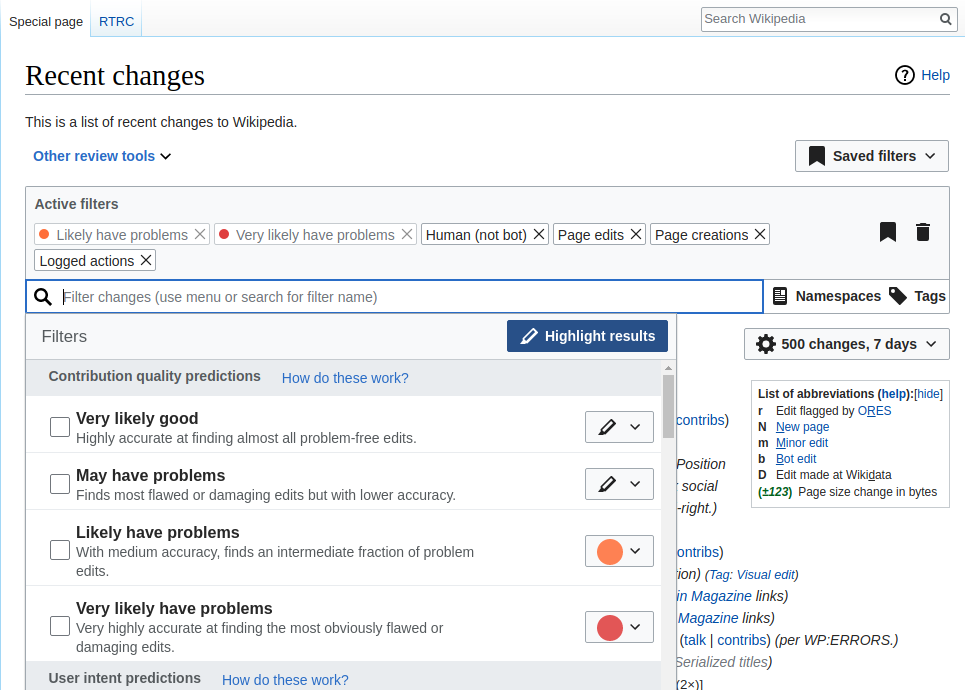
\includegraphics[width=.80\textwidth]{figures/Screenshot_of_Edit_review_filters}
  \caption{A screenshot of the Edit Review Filters interface with ORES score-based filters}
  \label{fig:edit_review_filters_screenshot}
\end{figure}

Many new tools have been developed since ORES has released that may not have been developed at all otherwise.  For example, the Wikimedia Foundation product department developed a complete redesign on MediaWiki's Special:RecentChanges interface that implements a set of powerful filters and highlighting.  They took the ORES Review Tool to it's logical conclusion with an initiative that they referred to as Edit Review Filters\footnote{\url{http://enwp.org/:mw:Edit_Review_Improvements}}.  In this interface, ORES scores are prominently featured at the top of the list of available features and they have been highlighted as one of the main benefits of the new interface to the editing community.

When we first developed ORES, English Wikipedia was the only wiki that we are aware of that had a robot that used machine prediction to automatically revert obvious vandalism\cite{carter2008cluebot}.  After we deployed ORES, several wikis developed bots of their own to use ORES predictions to automatically revert vandalism.  For example, in PatruBot in Spanish Wikipedia\footnote{\url{http://enwp.org/:es:Usuario:PatruBOT}} and Dexbot in Persian Wikipedia\footnote{\url{http://enwp.org/fa:User:Dexbot}} now automatically revert edits that ORES predicts are damaging with high confidence.  These bots have been received with mixed acceptance.  Because of the lack of human oversight, concerns were raised about PatruBot's false positive rate but after consulting with the developer, we were able to help them find an acceptable threshold of confidence for auto-reverts.

One of the most noteworthy new tools is the suite of tools developed by Sage Ross to support the Wiki Education Foundation's\footnote{\url{https://wikiedu.org/}} activities.  Their organization supports classroom activities that involve editing Wikipedia.  They develop tools and dashboards that help students contribute successfully and to help teachers monitor their students' work.  Ross has recently published about how they interpret meaning from ORES' article quality models\cite{ross2016visualizing} and has integrate this prediction into their tools and dashboards to recommend work that students need to do to bring their articles up to Wikipedia's standards.  See our discussion of interrogation in Section~\ref{sec:innovations_in_openness}.
